\begin{figure*}[t]
    \centering
    \begin{subfigure}[b]{0.02\textwidth}
        \center
        \begin{turn}{90} 
            \footnotesize
            Average Return
        \end{turn}
        \vspace{1.5cm}
    \end{subfigure}
    \begin{subfigure}[b]{0.3\textwidth}
        \center
        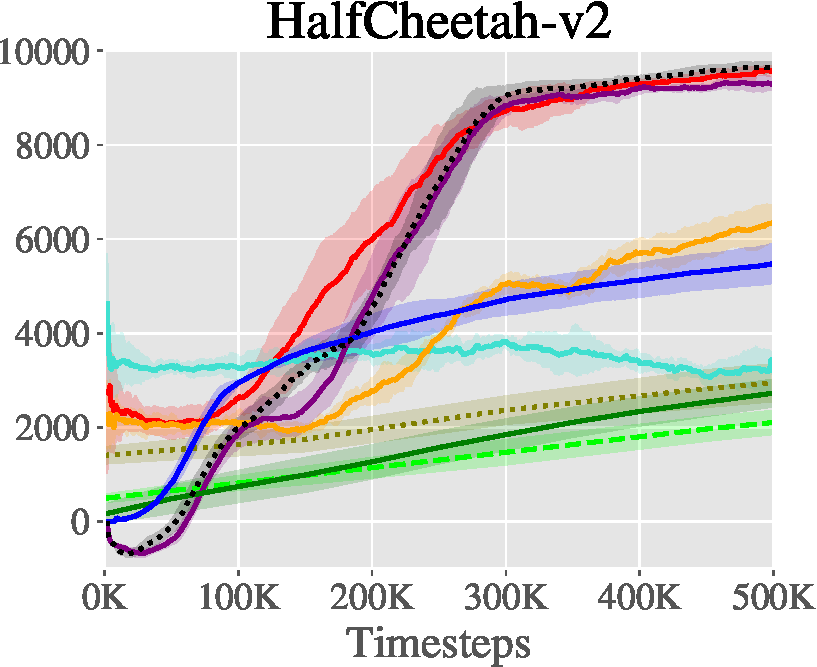
\includegraphics[width=\textwidth]{awac/figures/mujoco/hc-crop.pdf}
    \end{subfigure}
    \begin{subfigure}[b]{0.3\textwidth}
        \center
        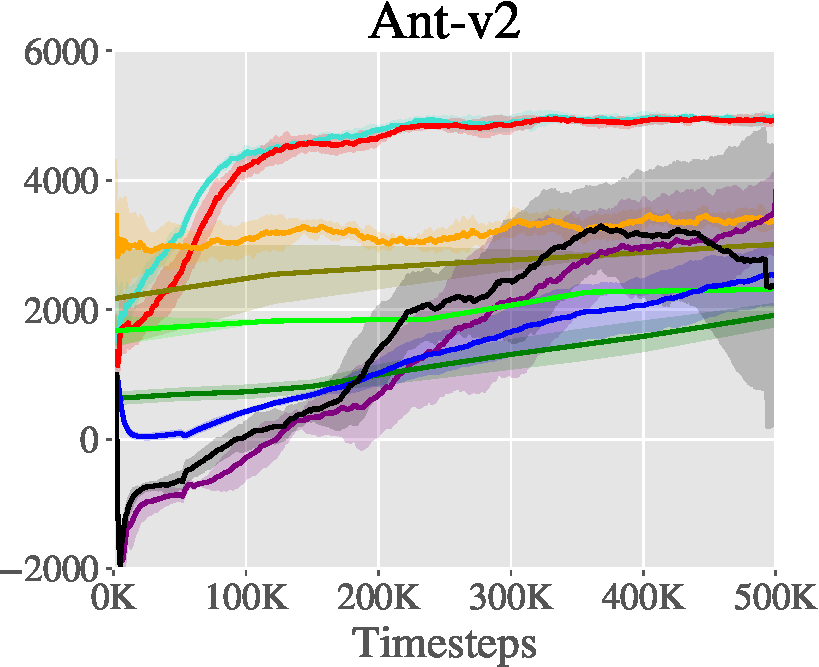
\includegraphics[width=\textwidth]{awac/figures/mujoco/ant-crop.pdf}
    \end{subfigure}
    \begin{subfigure}[b]{0.3\textwidth}
        \center
        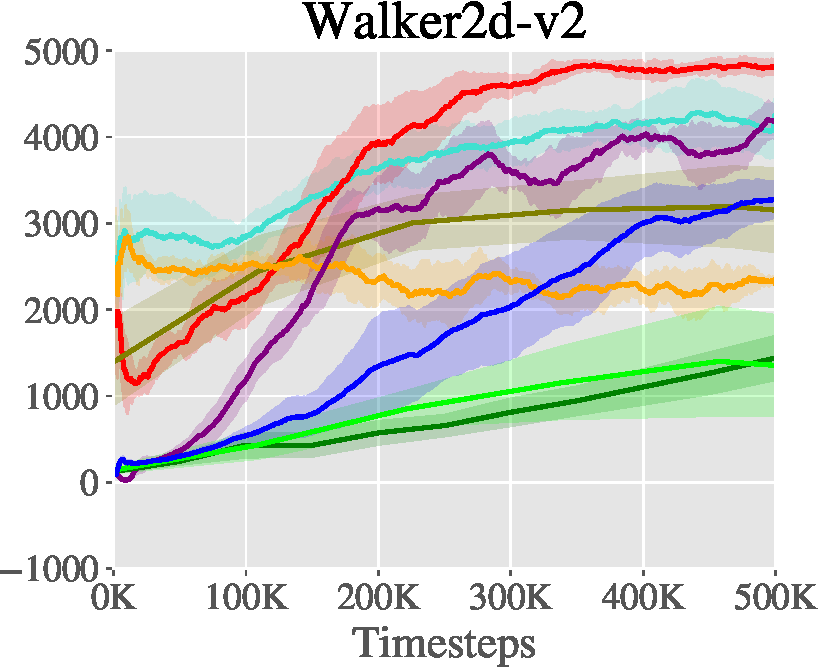
\includegraphics[width=\textwidth]{awac/figures/mujoco/walker-crop.pdf}
    \end{subfigure}
    
    \begin{subfigure}[b]{0.99\textwidth}
        \center
        % 
\includegraphics[width=1\textwidth]{awac/figures/mujoco/legend-crop.pdf}
        % 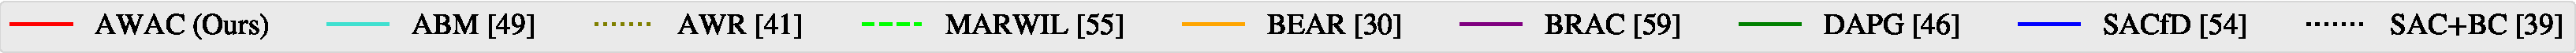
\includegraphics[width=1\textwidth]{awac/figures/mujoco/legend_ncol1-crop.pdf}
        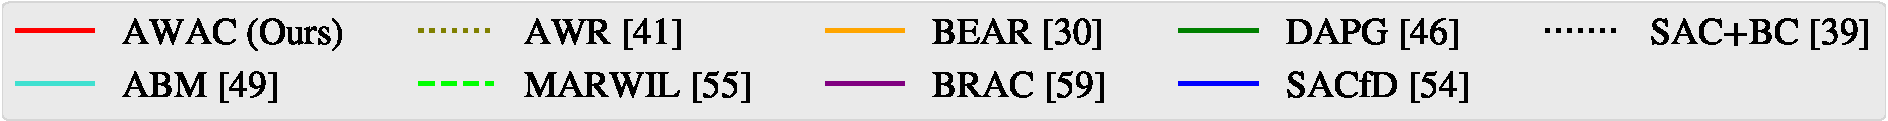
\includegraphics[width=0.6\textwidth]{awac/figures/mujoco/legend_ncol2-crop.pdf}
    \end{subfigure}
    \caption{
    % \footnotesize{
    Comparison of our method and prior methods on standard MuJoCo benchmark tasks. These tasks are much easier than the dexterous manipulation tasks, and allow us to better inspect the performance of methods in the setting of offline pretraining followed by online fine-tuning. SAC+BC and BRAC perform on par with our method on the HalfCheetah task, and ABM performs on par with our method on the Ant task, while our method outperforms all others on the Walker2D task. 
    Our method matches or exceeds the best prior method in all cases, whereas no other single prior method attains good performance on all of the tasks. }
    % }
    \label{fig:sim-learning-curves}
\end{figure*}